\chapter{Visualização de Software}\label{chap:visualizacao}

\textit{``Imagination or visualization, and in particular the use of diagrams,
has a crucial part to play in scientific research.''} René Descartes, 1637.

Há muita informação hoje disponível, circulando e com um fluxo de crescimento
exponencial. Grande parte dessa informação é útil para o ensino e a instrução.
Dados são recursos valiosos, porém é preciso compreendê-los \cite{messias2012}.

A visualização de um dado com propriedades visuais como posição, tamanho, forma
e cor, potencializam as habilidades sensoriais do ser humano. Possivelmente o usuário
irá extrair observações e conclusões sobre os dados, e também poderá moldar esse
conhecimento adquirido para atingir os objetivos \cite{card1999readings}
\cite{heer2012interactive} \cite{keim2002information}.

O estudo da visualização pode ser dividido em duas grandes vertentes, ambas
possuindo interação com usuário induzindo-o ao entendimento das informações
contidas nos dados \cite{de2003visual}:

\begin{enumerate}
  \item \textbf{Visualização Científica}: dados físicos e inerentemente
  geométricos;
  \item \textbf{Visualização de Informação}: informações não físicas, por
  exemplo coleções de documentos, podem ser beneficiadas, porém não há nenhuma
  forma óbvia de se mapear tais dados em uma imagem \cite{card1999readings}.
  Envolve algo mais complexo.
\end{enumerate}

Visualização da informação é portanto relacionada a \textbf{grandes conjuntos}
de dados. Um \textbf{conjunto} é um o número de atributos ou dimensões que o
identifica. Quantidade de dimensões é o mesmo que \textbf{dimensionalidade}.

Os tipos de dados comuns são: bidimensionais e multidimensionais
\cite{de2003visual}.

Os multidimensionais necessitam da aplicação de uma técnica
\cite{keim2002information}. São técnicas citadas por \citeonline{messias2012}:

\begin{itemize}
  \item Projeções geométricas:
	\begin{itemize}
		\item Coordenadas paralelas. Exemplo na Figura \ref{fig:parallel} \cite{kaichang2015};
	\end{itemize}
  \item Orientadas a pixel:
	\begin{itemize}
		\item \textit{recursive patterns};
		\item \textit{circle segments};
	\end{itemize}
  \item Iconográficas:
	\begin{itemize}
		\item \textit{stick figures};
	\end{itemize}
  \item Hierárquicas:
	\begin{itemize}
		\item \textit{Dimensional Stacking}.
	\end{itemize}
\end{itemize}

\begin{figure}[!htb]
  \centering
    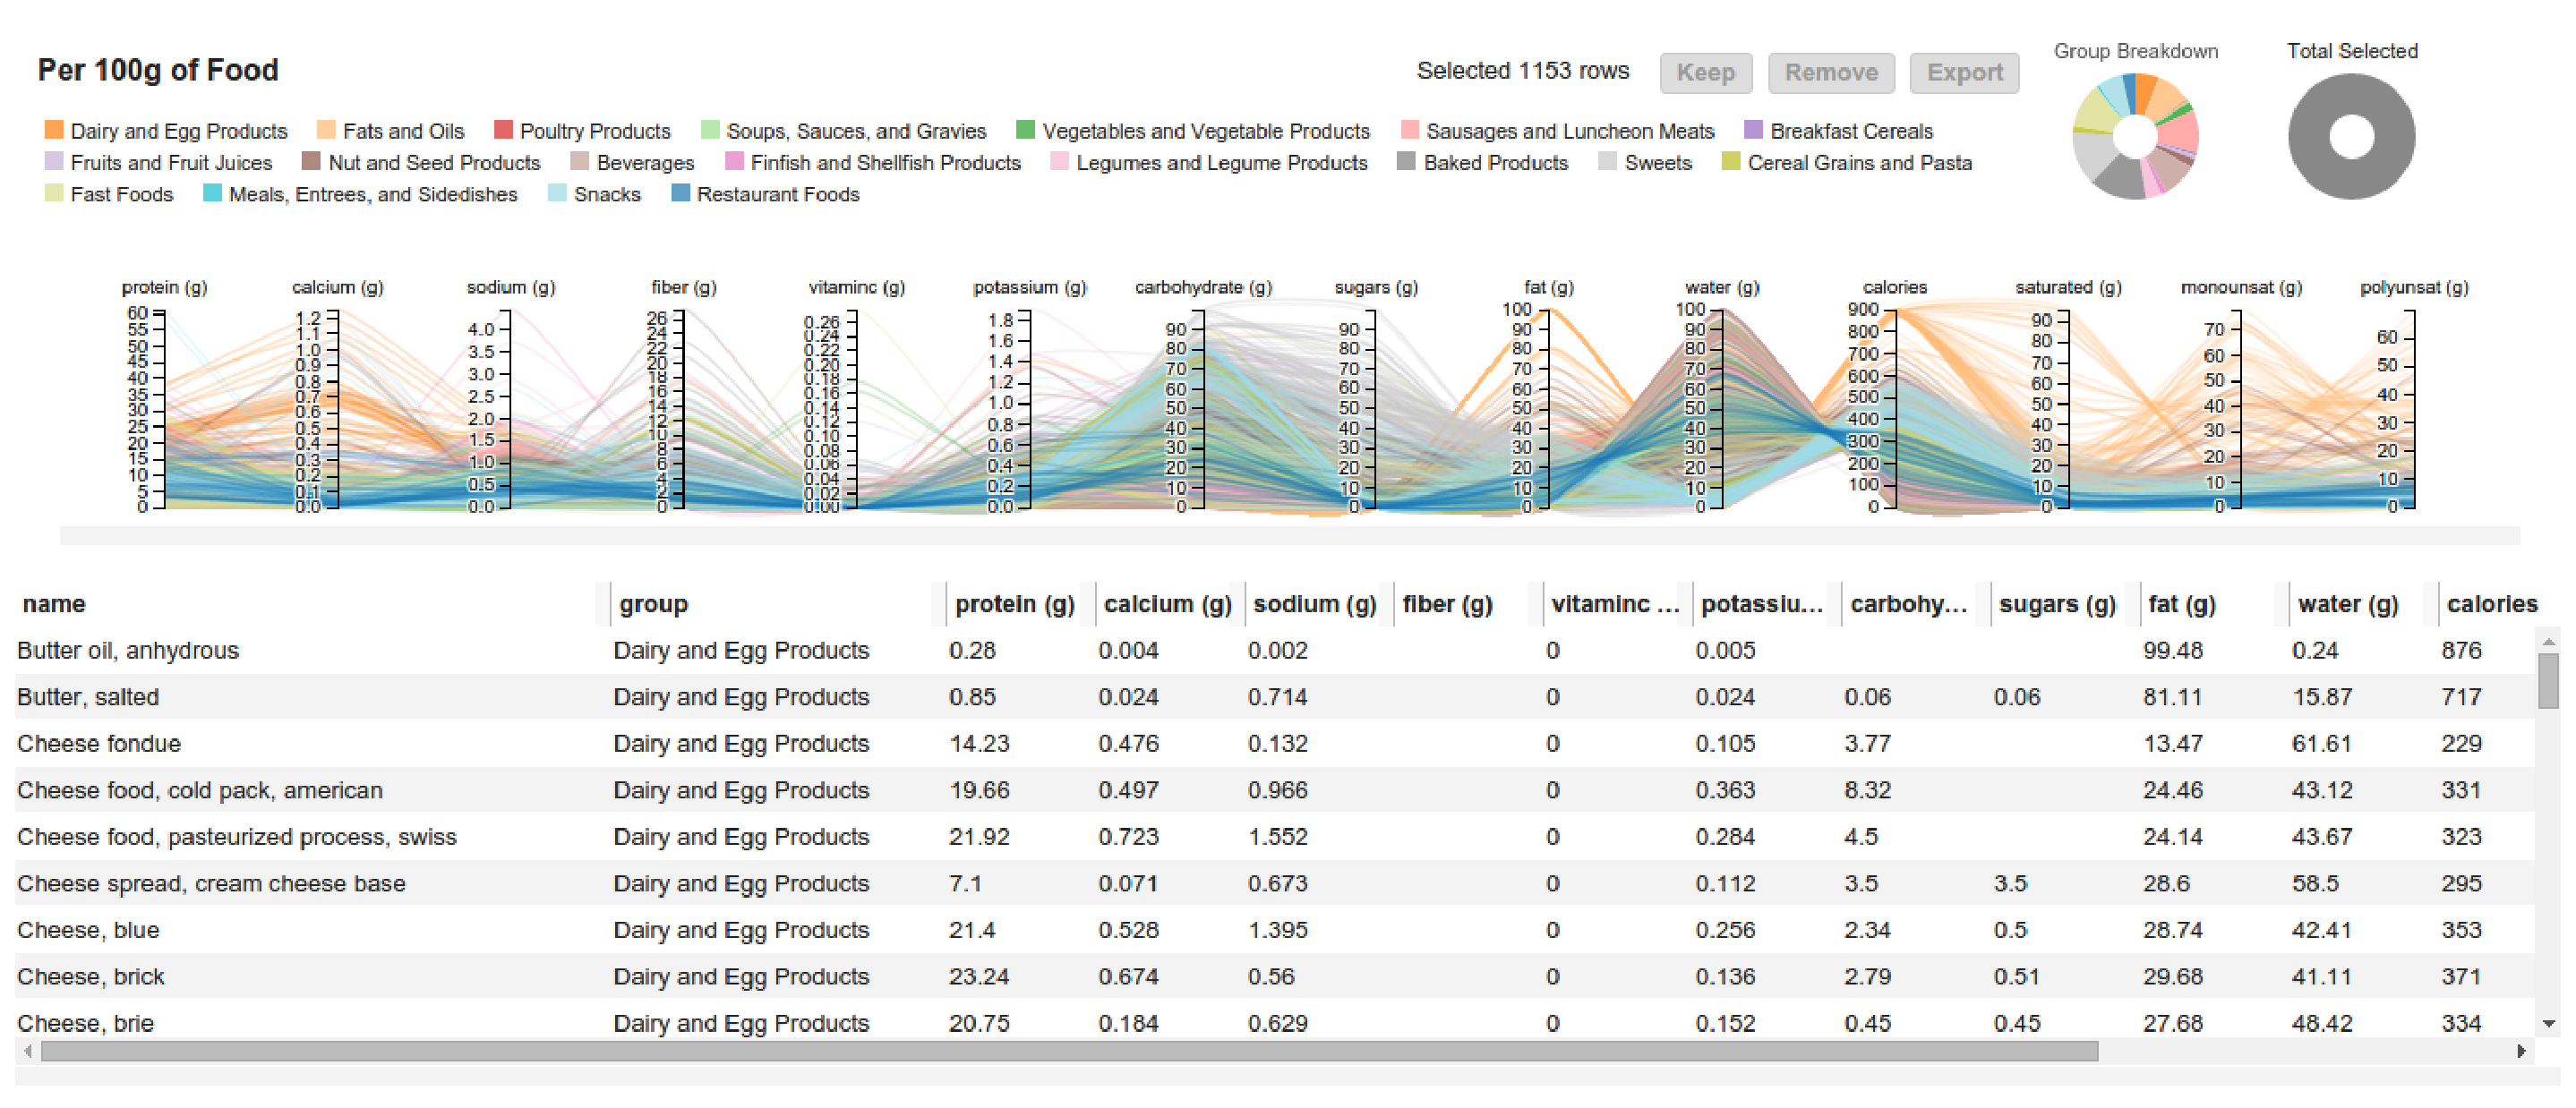
\includegraphics[keepaspectratio=true,scale=0.3]
    {figuras/parallel.eps}
  \caption{Exemplo de Coordenadas Paralelas}
  \label{fig:parallel}
\end{figure}

Portanto, segundo \citeonline{diehl2007software}, Visualização de Software
é uma subárea da Visualização de Informação. E os objetivos dela são: ``auxiliar
a compreensão de sistemas complexos de software e melhorar a produtividade do
processo de desenvolvimento'' \cite{messias2012}. É a representação gráfica de
aspectos técnicos, ou sociais, ou ambos de um software. As técnicas geram
exibições de aspectos do software que podem auxiliar tarefas de:

\begin{itemize}
	\item Gerenciamento;
	\item Projeto;
	\item Implementação;
	\item Depuração;
	\item Análise;
	\item Manutenção.
\end{itemize}

Visualização de Software é um dos braços da Visualização de Informação que mais
cresce \cite{telea2014data}. \citeonline{bassi2001software} apresentam alguns
benefícios de se utilizar ferramentas de VS:

\begin{itemize}
	\item Economia de tempo e dinheiro;
	\item Melhor compreensão;
	\item Aumento da produtividade;
	\item Auxílio na detecção de erros no código;
	\item Melhoria da qualidade.
\end{itemize}

\section{Categorias da Visualização de Software}

A visualização de software pode ser levada em consideração pelas três seguintes
categorias: estrutura, comportamento e evolução \cite{diehl2007software}.

\subsection{Estrutura}

Relacionada ao que é estático em um software, sem necessidade de executá-lo. Por
exemplo: o código-fonte, as estruturas de dados do programa, o grafo de chamadas
estático e a organização do sistema em módulos \cite{diehl2007software}.

Propriedades interessantes \cite{messias2012}:

\begin{itemize}
	\item Exatidão: linguagens de programação exacerbadamente definidas;
	\item Grande escala: sistemas que possuem uma quantidade grande de linhas
	de código;
	\item Relações e hierarquias entre entidades do código;
	\item Diversos atributos que expressam as características dessas entidades.
\end{itemize}

Ferramentas de geração de visualização da categoria estrutura compartilham o
mesmo modelo conceitual: a geração de um grafo que relaciona em seus vértices
as propriedades anteriormente citadas.

Exemplos de Visualização da estrutura de software: \textit{Team Assessment}
\cite{telea2009case} e \textit{CodeCity} \cite{wettel2008codecity}.

Uma técnica bastante elaborada, desenvolvida por \citeonline{holten2006hierarchical},
expressa em uma única imagem duas das propriedades: a estrutura hierárquica e
suas dependências internas (Figura \ref{fig:heb}).

\begin{figure}[!htb]
  \centering
    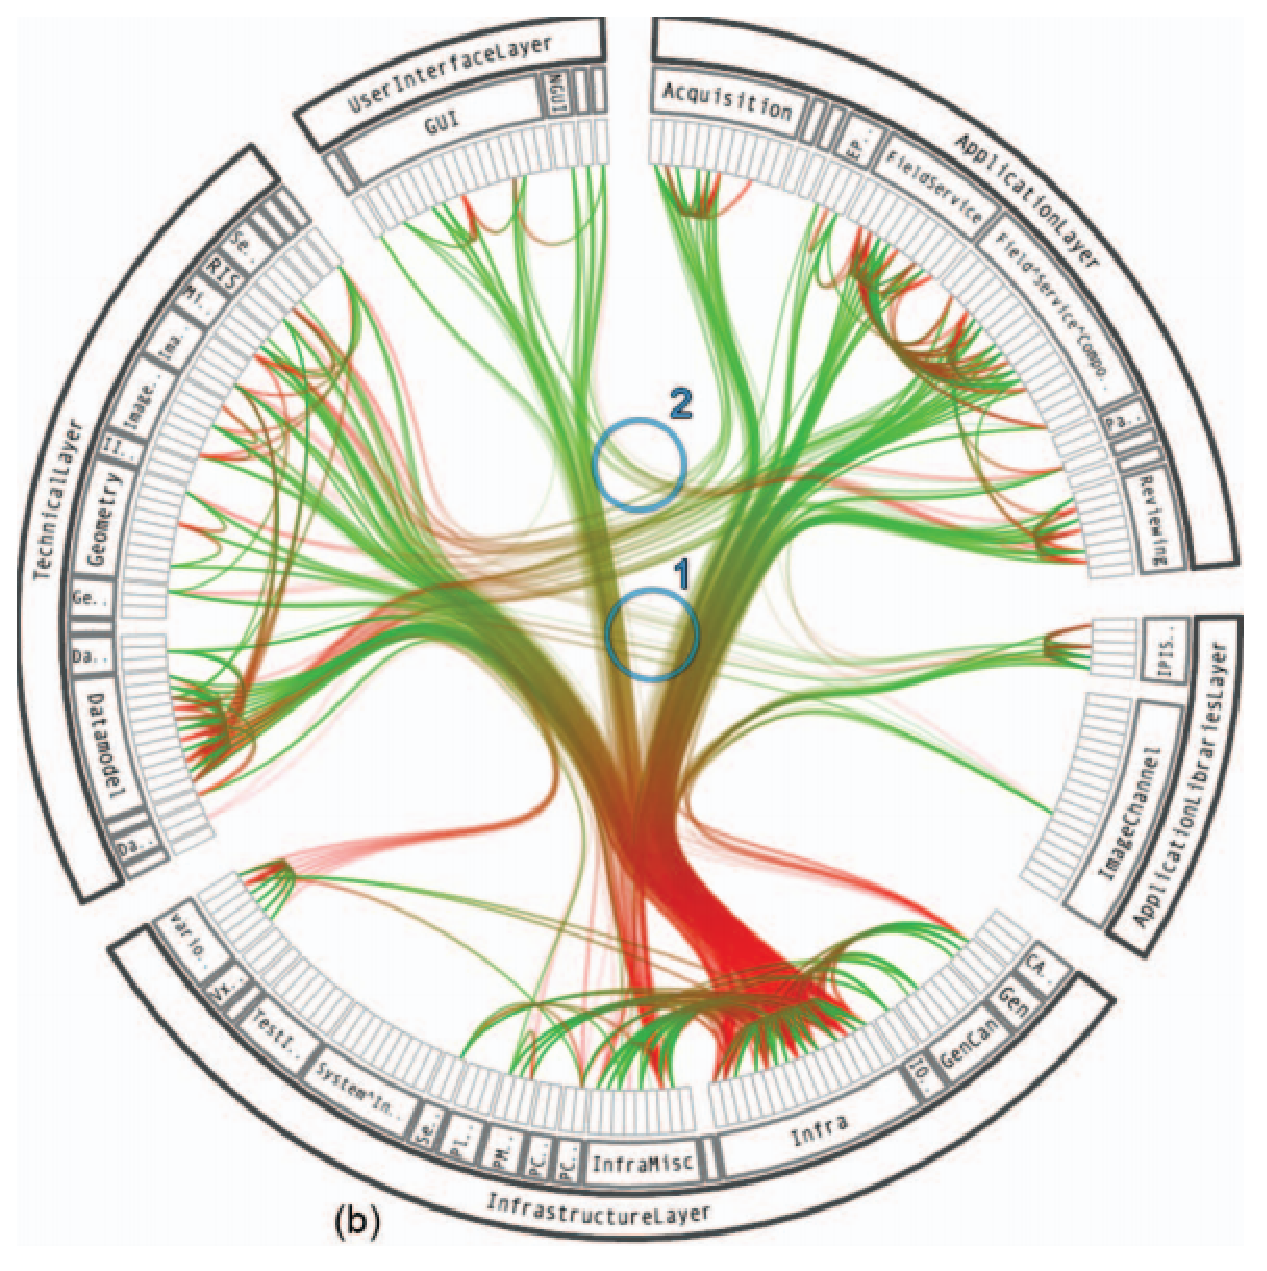
\includegraphics[keepaspectratio=true,scale=0.5]
    {figuras/heb.eps}
  \caption{Estrutura Hierárquica \cite{holten2006hierarchical}}
  \label{fig:heb}
\end{figure}

Métricas podem ser incluídas em visualizações da estrutura. Na ferramenta
SolidSX (Figura \ref{fig:solidSX}), \citeonline{reniers2011visual} inclui
algumas métricas como linhas de código, comentários e complexidade. Essa
ferramenta une três técnicas:

\begin{itemize}
	\item \textit{TreeMap} - disposição das hierarquias do código;
	\item \textit{HEB};
	\item \textit{TableLens} - módulos são linhas e métricas são colunas de uma
	tabela, mapeando as métricas e destacando-as por cores.
\end{itemize}

\begin{figure}[!htb]
  \centering
    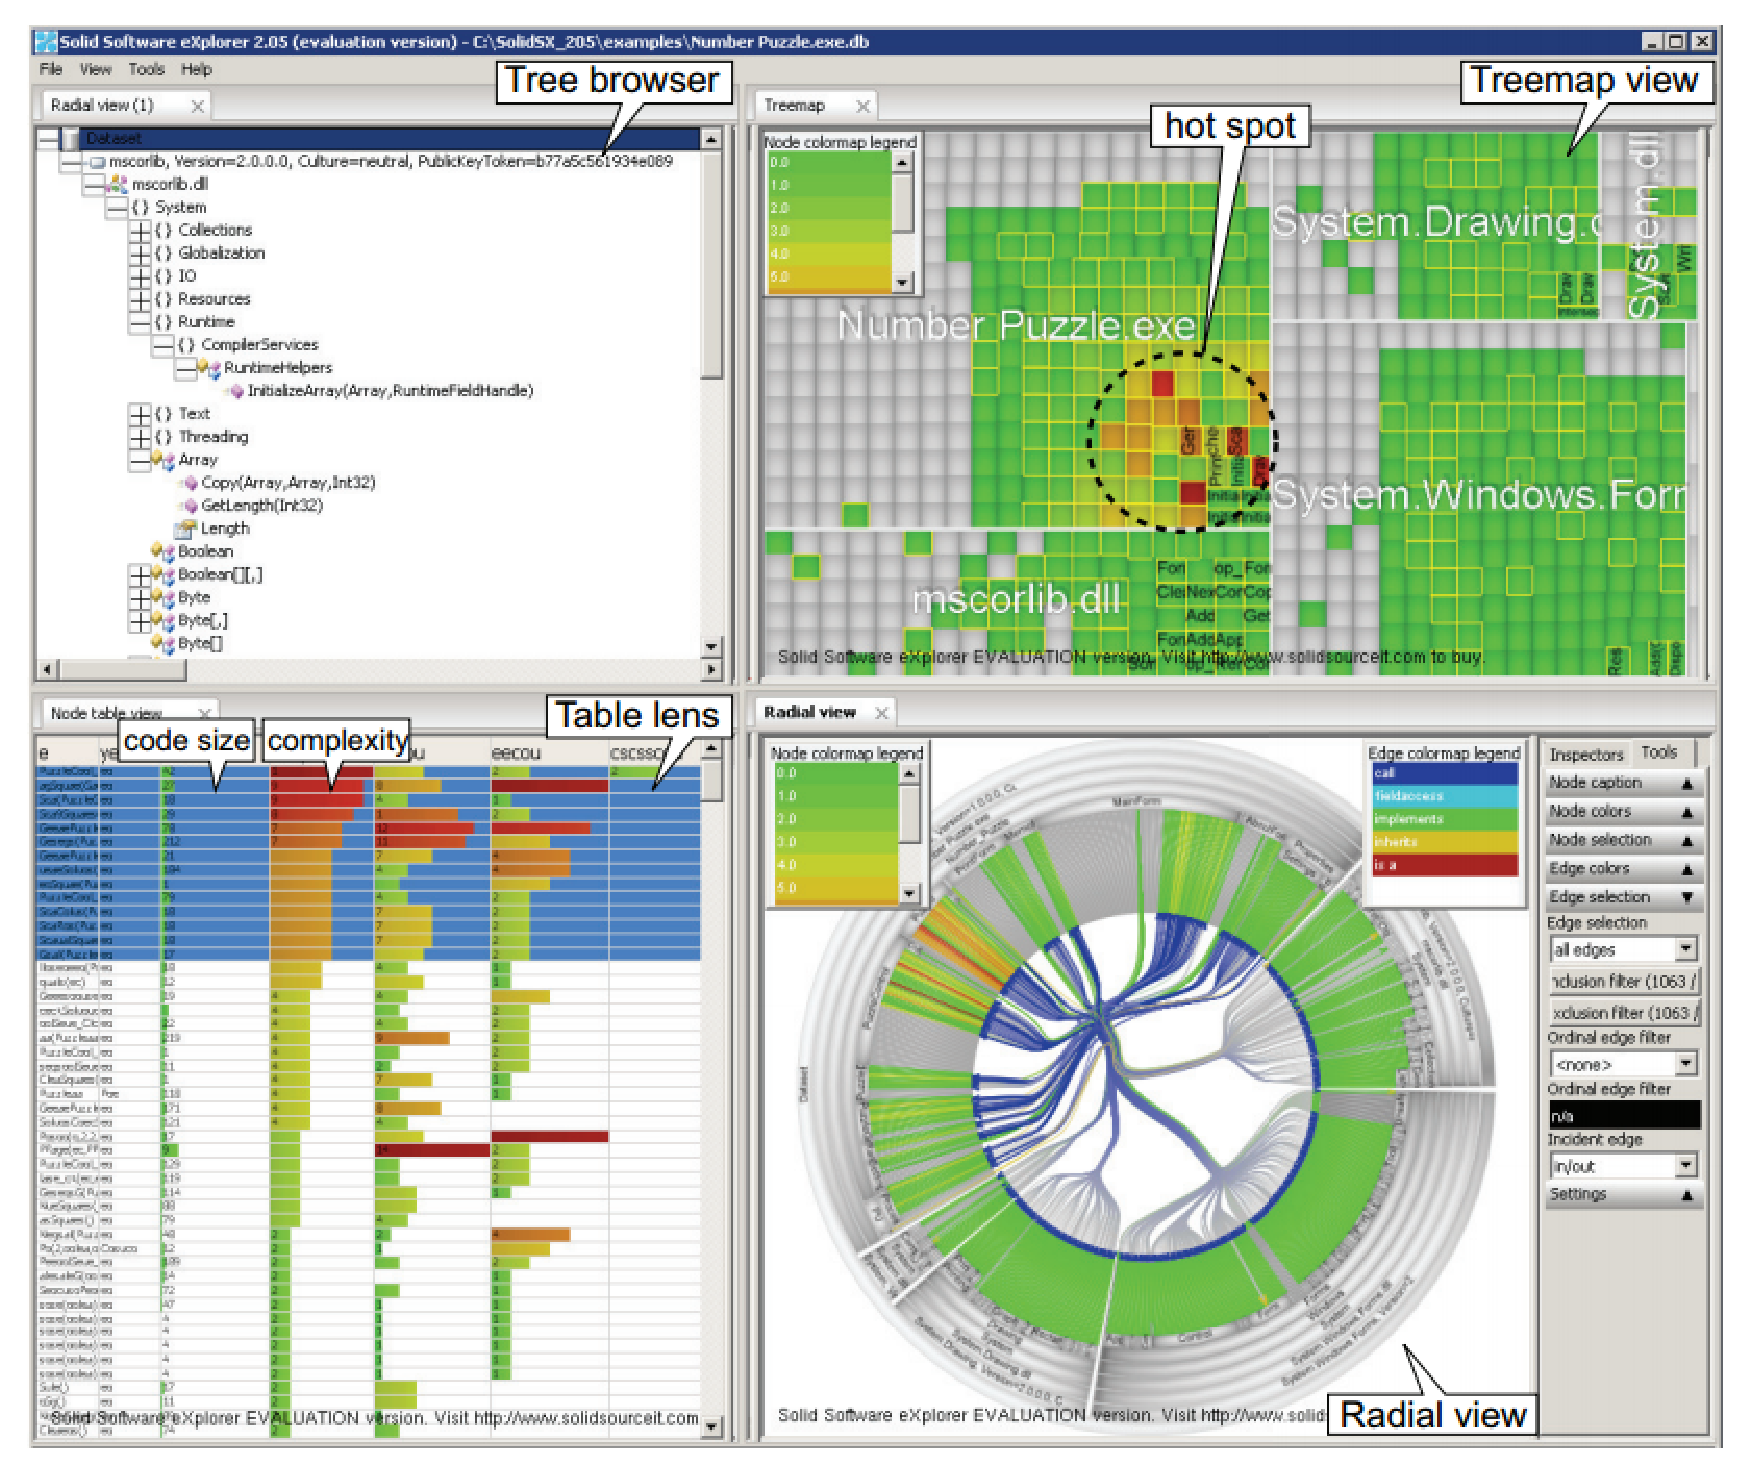
\includegraphics[keepaspectratio=true,scale=0.5]
    {figuras/solidSX.eps}
  \caption{Ferramenta SolidSX \cite{reniers2011visual}}
  \label{fig:solidSX}
\end{figure}

\subsection{Comportamento}

Nesta categoria o software é executado. Análise do que acontece, em tempo de execução, dada
determinada entrada. Técnica: sequência de estado. Combinar dados e código para
analisar interação com a memória. Dependendo do paradigma de programação, pode
haver uma relação entre os métodos ou funções e a comunicação entre os objetos
\cite{cornelissen2009systematic} \cite{diehl2007software}.

Aplicações dessa categoria:

\begin{itemize}
	\item Análise de traces de execução;
	\item Visualização dinâmica e recuperação de arquitetura;
	\item Animação de algoritmos;
	\item Depuração visual;
	\item Apoio visual à atividade de teste.
\end{itemize}

Exemplo da ferramenta \textit{Tarantula} \cite{jones2002visualization} -
Depuração visual, execução de testes, destaque com escala que vai de vermelho
(falha) até verde (sucesso).

\subsection{Evolução}

Categoria aplicada para compreensão das modificações ao longo do tempo. A
manutenção e evolução de um sistema pode chegar a 80\% do custo total de
desenvolvimento \cite{pfleeger2005analyzing}. Dado este que fortalece as
visualizações desta categoria.

\citeonline{biggerstaff1993concept} dizem que: ``Uma pessoa entende um programa
quando ele ou ela é capaz de explicar o programa, a estrutura, o seu
comportamento, os efeitos no seu contexto operacional, e os seus relacionamentos
com o domínio da aplicação em termos que são qualitativamente diferentes dos
\textit{tokens} usados para a construção do código-fonte do programa.'' Essa
definição de entendimento se alinha com as duas primeiras categorias do estudo
de visualização, e entender a evolução de software pode ser igualmente
importante como entender sua estrutura, considerando aspectos gerenciais e
administrativos também.

\section{Proposta de VS para o Mezuro}

Como possível evolução do Mezuro, é proposto o levantamento de um determinado
número de visualizações que serão submetidas a avaliação por desenvolvedores da
Universidade de Brasília - Faculdade Gama, e outros desenvolvedores envolvidos
com o Mezuro, por meio de questionário. Logo, será proposto o estudo deste
questionário, análise das respostas e sugestões, e a ampla divulgação dos
resultados à comunidade do Mezuro.

Estas visualizações estarão disponíveis por meio de uma aplicação Rails com
páginas estáticas, exceto aquelas visualizações que possuem algum tipo de
interação com o usuário, por meio de cliques ou outras ações.

A proposta, portanto é a especificação de visualizações e técnicas que podem ser
aplicadas ao Mezuro.

\section{Trabalhos Relacionados}

No artigo \textit{CodeCrawler – An Extensible and Language Independent 2D and
3D Software Visualization Tool}, \citeonline{lanza2005codecrawler}
desenvolveram uma ferramenta para visualização de software capaz de exibir
detalhes de uma forma polimétrica, que é capaz de mostrar informações como as
métricas do software, sua semântica e a relação entre as classes, por exemplo.
Segundo o autor, essa visualização pode ser aplicada em vários contextos e não
somente em aspectos de software. Idealmente, a ferramenta é capaz de gerar
visualizações para software com grande número de linhas código. Porém é levado
em consideração a integração das visualizações em IDEs e essa solução não é
explorada. A utilização da técnica em diferentes ferramentas também não é
discutida.

Os autores, \citeonline{dosvisualizacc}, do \textit{Visualização de Software
Como Suporte ao Desenvolvimento Centrado em Métricas Orientadas a Objetivos}
criaram um plugin escrito em C++ para visualização de métricas OO, que são
coletadas pela ferramenta Qt Creator\footnote{\url{http://www.qt.io/ide/}}. As
métricas definidas foram: média de atributos por métodos em uma classe (MAC);
quantidade de métodos por classe (QMC); tamanho dos métodos por classe (TMC);
quantidade de atributos por classe (QAC); e quantidade de métodos públicos
(QMC). Métricas essas relacionadas com a categoria \textbf{estrutura} da VS.
E nesse plugin os casos de uso ou funcionalidades
são: calcular métricas: QAC; QMC; MAM; TMC; QMP. Além da
possibilidade de calcular a média das métricas, obter detalhes das métricas e
obter ajuda sobre as métricas. Um dos pontos importantes destacados no
resultado é a observação de que é possível garantir certo nível de qualidade
utilizando essas métricas até mesmo para projetos pequenos, com duas ou três
classes.

Porém a ferramenta só gera visualizações para aplicações escritas em C++, que é
um fator limitante devido à incorporação do plugin à ferramenta Qt Creator. O
plugin calcula também apenas cinco métricas consideradas fundamentais para
avaliar a qualidade de um software. E o detalhamento de determinada classe e
uma visualização da evolução do projeto em uma linha do tempo também não foram
abordados neste trabalho.

O artigo dos autores \citeonline{ramosanalise}, cujo o título é \textit{Análise de
Métricas Estáticas para Sistemas JavaScript}, não trata necessariamente de
visualização de software, embora em várias figuras mostrem distribuições dos
projetos e seus respectivos valores das métricas escolhidas. Portanto,
destacamos a escolha da ferramenta
\textit{https://github.com/jared-stilwell/escomplex}\footnote{\url{https://github.com/jared-stilwell/escomplex}},
que analisa métricas de projetos escritos em JavaScript (linguagem que ainda
não é suportada para análise no Mezuro), e escolha das métricas que são: número
de módulos; linhas de código; número de parâmetros; complexidade ciclomática;
densidade de complexidade ciclomática; métricas de complexidade de Halstead; e
índice de manutenção.

É importante ressaltar também o artigo \textit{Understanding software evolution
using a combination of software visualization and software metrics}. Os
autores, \citeonline{Lanza02understandingsoftware}, ressaltam que há uma grande
quantidade de dados hoje em circulação nos sistemas informatizados. Consideram ser este um
dos maiores problemas nas pesquisas de evolução de um software, e em alguns
casos as várias versões destes sistemas precisam ser analisadas em paralelo.
Então, considerando esta complexidade, uma técnica que pode auxiliar na
abordagem destas pesquisas é a visualização de software. É comentado sobre a
capacidade humana de observação de múltiplos aspectos de um problema em
paralelo e sua ligação direta com a visualização e o auxílio que possivelmente
esta trará o entendimento do sistema.

A técnica visual utilizada foi a matriz de evolução: combina visualização de
software com suas métricas \cite{lanza2001evolution}. Esta técnica permite
observar classes que merecem atenção, por exemplo, por terem crescido ou
encolhido durante a vida útil do sistema. E a abordagem apresentada é
independente da linguagem, mesmo que em um dos estudos de caso tenha sido
analisado um software escrito em Smalltalk.

Dissertando um pouco mais sobre a técnica, \citeonline{Lanza02understandingsoftware}
mostram suas minúcias. Cada coluna representa as diferentes versões do
software. Cada linha representa uma classe. E nessa técnica há algo importante
para este trabalho de conclusão de curso, onde é desejável trabalhar com o
software e a evolução do mesmo durante certo tempo ou período.

Características que podem ser observadas na técnica:

\begin{itemize}
  \item Tamanho dos sistemas em termos de classes. Quanto mais linhas, maior o
  sistema;
  \item Classes adicionadas e removidas;
  \item Períodos de decréscimo, estabilização ou crescimento do sistema durante a
  sua ``evolução''
  \item Classes \textit{Dayfly}. Classes com um tempo de vida pequeno, por
  exemplo que apenas apareceram em uma única versão do sistema;
  \item Classes que se mantêm (o contrário da característica observada no ponto
  anterior).
\end{itemize}

Porém, no artigo foi constatado que essa representação não é precisa o suficiente.
A evolução então seria o uso das métricas de código-fonte.

A Figura \ref{fig:evolutionMatrixAspects} \cite{Lanza02understandingsoftware}
foi extraída do artigo e mostra essas características ou aspectos na evolução de
um sistema, utilizando a técnica da matriz de evolução.

\begin{figure}[!htb]
  \centering
    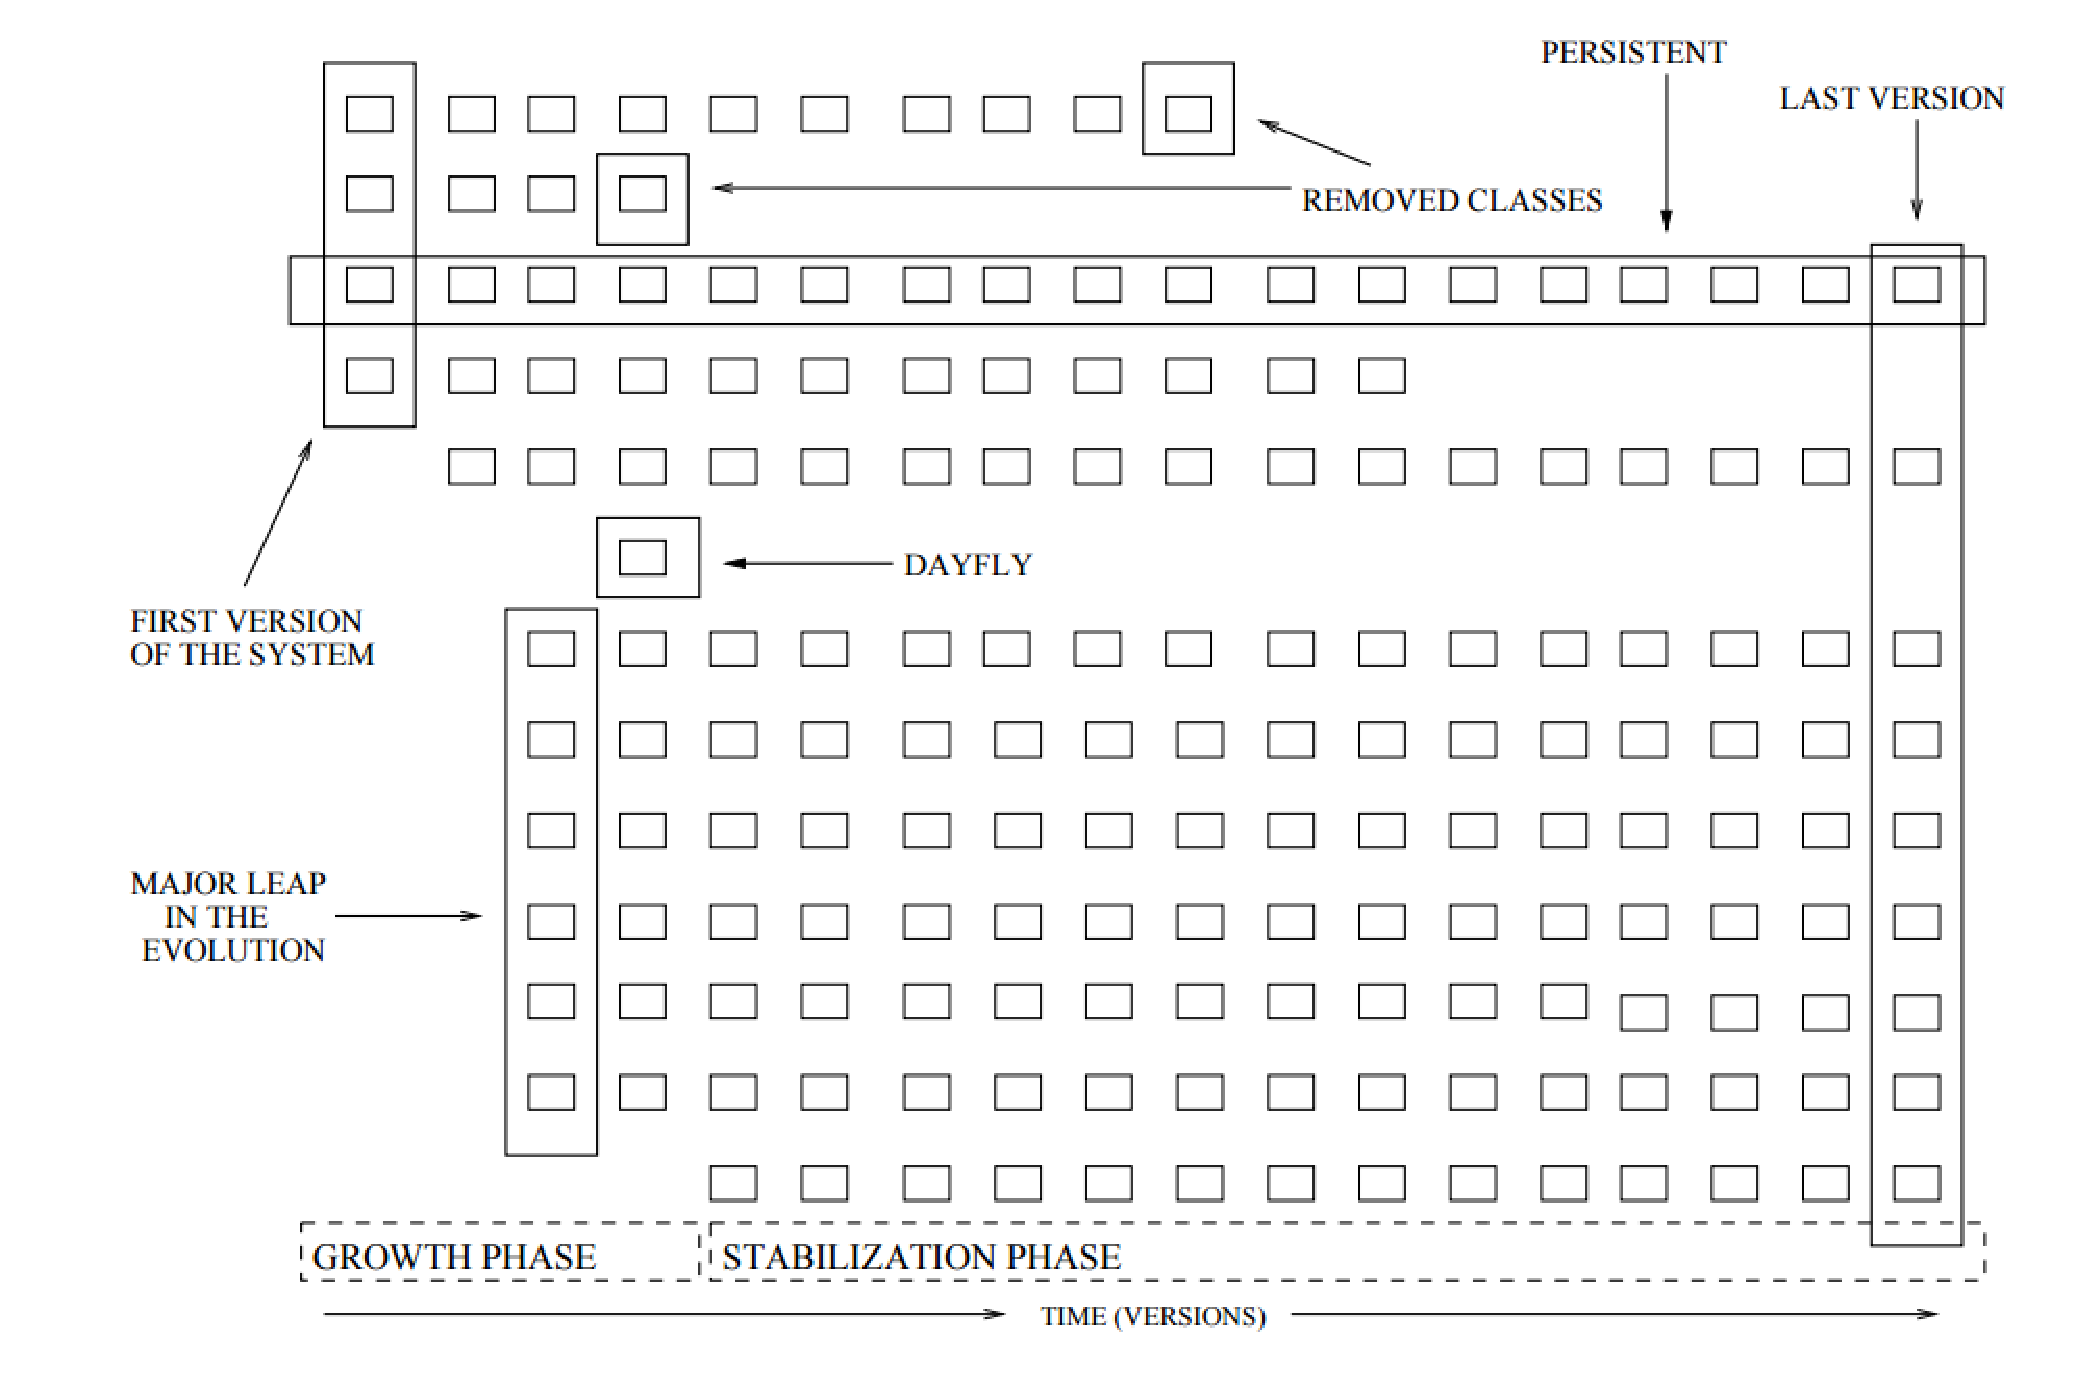
\includegraphics[keepaspectratio=true,scale=0.5]
    {figuras/evolutionMatrixAspects.eps}
  \caption{Aspectos da evolução de um sistema utilizando Matriz de Evolução}
  \label{fig:evolutionMatrixAspects}
\end{figure}


Ainda comentando sobre o artigo \textit{Understanding software evolution using
a combination of software visualization and software metrics}, destacamos
o modo como foi inserida esta evolução da utilização das métricas de código-fonte:
altura e largura das caixas na visualização representam métricas das
classes. Métricas utilizadas: número de métodos (\textit{NOM}) e número de
atributos (\textit{NOA}).

E com as métricas definidas, foi feita uma categorização das classes em:

\begin{itemize}
  \item \textit{Pulsar}: uma classe que cresce e diminui durante o ciclo de
  vida do sistema;
  \item \textit{Supernova}: classe que de repente cresce bastante;
  \item \textit{White Dwarf}: classe que era grande, mas por algum motivo as
  suas responsabilidades foram divididas em outras classes e esta diminui;
  \item \textit{Red Giant}: é uma classe considerada \textit{god class}
  \cite{riel1996object}, por muito tempo, ou seja: uma classe grande que
  implementa muitas funcionalidades;
  \item \textit{Idle}: classe constante, inativa, sem grandes modificações.
\end{itemize}

Concluindo, o artigo apresenta uma abordagem útil que talvez auxilie no
entendimento de um sistema. Porém é abordado no mesmo uma quantidade de
métricas pequena (embora significativa para o contexto). Outro ponto negativo é
que em sistemas mui grandes, a visualização pode esbarrar em limitações de
exibição em uma única tela. E a abordagem pode apresentar problemas com nomes
repetidos de classes (considerando que este pode ser ou não um erro no
desenvolvimento de um sistema).
